\documentclass[11pt, oneside]{article}   	% use "amsart" instead of "article" for AMSLaTeX format
\usepackage{geometry}                		% See geometry.pdf to learn the layout options. There are lots.
\geometry{letterpaper}                   		% ... or a4paper or a5paper or ...
%\geometry{landscape}                		% Activate for rotated page geometry
%\usepackage[parfill]{parskip}    		% Activate to begin paragraphs with an empty line rather than an indent
\usepackage{graphicx}				% Use pdf, png, jpg, or eps§ with pdflatex; use eps in DVI mode
								% TeX will automatically convert eps --> pdf in pdflatex
\usepackage{amssymb}
\usepackage{amsmath}
\usepackage{gensymb}

%SetFonts

%SetFonts


\title{Brief Article}
\author{The Author}
%\date{}							% Activate to display a given date or no date

\begin{document}

\section{Situation}

\subsection{Simulation}

La simulation se d\'eroule sur un temps $T$ ($t \in [0, T[$).
La vitesse de rotation en longitude de la Terre est $v_{\mathit{Terre}}$.

\subsection{Des satellites}

On dispose de plusieurs satellites $S$ qui orbitent autour de la terre. \\*

Chaque satellite $s \in S$ est d\'efini par :

\begin{itemize}
\item sa position (latitude, longitude) au temps $t$ : $P_{s, t} = (\varphi_{s, t}, \lambda_{s, t})$
\item sa vitesse en latitude $v_{s, t}$ ($100 \leq |v_{s,t}| \leq 500$)
\item l'orientation de la cam\'era au temps $t$ : $(\Delta\varphi_{s, t}\, \Delta\lambda_{s, t})$
\item la vitesse maximale de rotation de la cam\'era sur les deux directions $w_s$
\item l'orientation maximale de la cam\'era dans les deux directions $d_s$
\end{itemize}

On peut mettre par \'ecrit plusieurs \'equations qui d\'efinissent l'\'evolution de la cam\'era dans le temps, pour tout $t$ :

\begin{equation}
-d_s \leq \Delta\varphi_{s, t} \leq d_s
\label{max-phi}
\end{equation}

\begin{equation}
-d_s \leq \Delta\lambda{s, t} \leq d_s
\label{max-lambda}
\end{equation}

\begin{equation}
\Delta\varphi_{s, t+1} \in [-w_s\Delta\varphi_{s, t}, w_s\Delta\varphi_{s, t}]
\label{max-speed-phi}
\end{equation}

\begin{equation}
\Delta\lambda_{s, t+1} \in [-w_s\Delta\lambda_{s, t}, w_s\Delta\lambda_{s, t}]
\label{max-speed-lambda}
\end{equation}

L'\'evolution de la position du satellite $s$ dans le temps, pour tout $t$ :

\begin{equation}
\begin{displaystyle}
\text{La latitude } \varphi_{s, t+1} =
	\begin{cases}
		\varphi_{s, t} + v_s & \mathit{si} -90\degree \leq \varphi_{s, t} + v_s \leq 90\degree \\
		180\degree - (\varphi_{s, t} + v_s) & \mathit{si} \ \varphi_{s, t} + v_s > 90\degree \footnotemark \\
		-180\degree - (\varphi_{s, t} + v_s) & \mathit{si} \ \varphi_{s, t} + v_s < -90\degree \footnotemark \\
	\end{cases}
\end{displaystyle}
\end{equation}

\addtocounter{footnote}{-1}
\footnotetext{On passe par dessus le p\^ole Nord}
\stepcounter{footnote}
\footnotetext{On passe par dessus le p\^ole Sud}

\begin{equation}
\begin{displaystyle}
\text{La longitude }\lambda_{s, t+1} =
	\begin{cases}
		\lambda_{s, t} + v_{Terre} & \mathit{si} -90\degree \leq \varphi_{s, t} + v_s \leq 90\degree \\
		-180\degree - (\lambda_{s, t} + v_{Terre}) & \mathit{si} \ \varphi_{s, t} + v_s > 90\degree \\
		-180\degree - (\lambda_{s, t} + v_{Terre}) & \mathit{si} \ \varphi_{s, t} + v_s < -90\degree
	\end{cases}
\end{displaystyle}
\end{equation}

\begin{equation}
\begin{displaystyle}
\text{La vitesse } v_s =
	\begin{cases}
		v_s & \mathit{si} -90\degree \leq \varphi_{s, t} + v_s \leq 90\degree \\
		-v_s & \mathit{si} \ \varphi_{s, t} + v_s > 90\degree \\
		-v_s & \mathit{si} \ \varphi_{s, t} + v_s < -90\degree
	\end{cases}
\end{displaystyle}
\end{equation}

Les seules variables du probl\`emes sont donc l'orientation de la cam\'era du satellite au temps $t+1$.

\subsection{Des collections}

On dispose d'une liste de collections $C$. \\

Chaque collection $c \in C$ est d\'efinie par :

\begin{itemize}
\item une valeur de score $score_c$
\item une liste de points \`a capturer  $P_c = [(\varphi_1, \lambda_1), (\varphi_2, \lambda_2), ...]$
\item une liste d'intervalles de temps dans lesquels il est possible de capturer les points
$R_c = [[t_1, t_2], [t_3, t_4], ...]$
\end{itemize}

%-----------------

\section{Le probl\`eme}

Posons $X$ la listes des points captur\'es : $X = [(x, s, t), ...]$\footnote{Ici un point $x = (\varphi, \lambda)$ captur\'e par le satellite $s$ au temps $t$}

On cherche \`a maximiser le score avec

\begin{equation}
	\mathit{score} = \sum_{c \; \in \; C_{\mathit{prises}}} \mathit{score}_c
\end{equation}

$C_{\mathit{prises}}$ repr\'esente les collections ``prises'', c'est \`a dire les collections dont on a photographi\'e tous les points.

\begin{equation}
	C_{\mathit{prises}} = \{ c \ | \ c  \in  C \;�\mathit{et} \ \forall p \in P_{c} \ \exists (x, s, t) \in X \ \mathit{tq} \ x = p \}
\end{equation}

o\`u

$C$ : l'ensemble des collections

$P_{c}$ : les points de la collection $c$

$X$ : les points captur\'es \\

D\'efinissons $X$, l'ensemble des points captur\'es :

\begin{equation}
	X = \{ p \ | \ p \ \in \ \underset{c \ \in \ C}\cup P_{c} \ \mathit{et} \ p \;� \text{``a \'et\'e captur\'e''} \}
\end{equation}

On dit que $p$ ``a \'et\'e captur\'e'' si :

\begin{equation}
	\exists s \in S, \ \exists t \in [0, \, t_{max}[ \ \mathit{tel \, que} \ p = (\varphi_{s, t} + \Delta\varphi_{s, t}, \, \lambda_{s, t} + \Delta\lambda_{s, t})
\end{equation}

\emph{ie.} il existe un satellite $s$ qui a prit $p$ en photo au temps $t$.

% --------

\section{Id\'ees}

\subsection{Algorithme g\'en\'etique}

Puisque que les seules valeurs que nous pouvons influencer concernent
l'orientation de la cam\'era de chaque satellite, les solutions au probl\`eme
ressemblent \`a la liste des mouvements des cam\'eras permettant d'effectuer le
meilleur score. \\

Pour chaque cam\'era, on peut donc cr\'eer une table de cette fa\c{c}on :

\begin{table}[htb]
\begin{center}
\begin{tabular}{ l | r r}
	temps & D\'ecalage $\Delta\varphi$ & D\'ecalage $\Delta\lambda$ \\
	\hline
 	0 & 0 & 0 \\
	1 & +2 & -1 \\
	2 & +10 & -1 \\
	 \multicolumn{3}{l}{...} \\
	T-1 & -2 & +3 \\
\end{tabular}
\end{center}
\caption{\label{tab:mouvements}Mouvements de la cam\'era du satellite 1.}
\end{table}

On cr\'eerait donc des individus poss\'edant autant de tables qu'il y a de
satellites et on les ferait \'evoluer \`a la recherche d'une solution optimale.

Les d\'ecalages $\Delta\varphi$ et $\Delta\lambda$ ne prennent pas n'importe
quelle valeur. On doit respecter les contraintes exprim\'ees dans les
\'equations \eqref{max-phi} \eqref{max-lambda} \eqref{max-speed-phi}
\eqref{max-speed-lambda}. \\

Reste \`a d\'efinir mutations et croisements.

Une mutation peut consiter en l'addition ou la soustraction de $1$ sur une case
d'une des tables d'un individu, tant que la nouvelle position reste valide.

Le croisement pose probl\`eme car on va certainement cr\'eer une solution
interdite.
L'id\'ee la plus simple pour croiser deux individus $x_1$ et $x_2$ est
certainement de s\'electionner un m\^eme satellite $s$ dans chaque et de croiser sa
table de mouvements (\emph{ie} la d\'ecouper au temps $t_k$ et \'echanger deux
morceaux afin de cr\'eer $x_1'$ et $x_2'$). La ligne $t_{k+1}$ dans les tables
est probablement incompatible avec la ligne $t_k$ (vitesse trop grande,
d\'epassement de la borne $d_s$).

\subsubsection{Mod\'eliser les mouvements par un graphe}

\`A garder en t\^ete.

\begin{figure}[htb]
    \begin{center}
        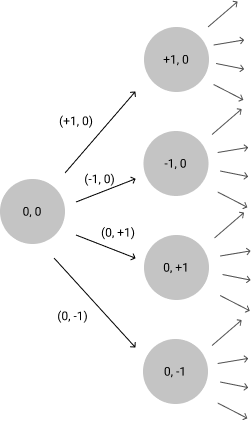
\includegraphics[scale=0.5]{graph.png}
        \caption{Mod\'elisation des valeurs que peut prendre une ligne de la table
        \ref{tab:mouvements}}
    \end{center}
\end{figure}

En fonction du mouvement pr\'ec\'edent, certains mouvement deviennent interdits car
ils vont mettre en d\'efaut les \'equations \eqref{max-phi} \eqref{max-lambda}
\eqref{max-speed-phi} \eqref{max-speed-lambda}.

\subsection{Recuit simul\'e}

\end{document}
